\documentclass[12pt]{article}

% Packages for figures and geometry
\usepackage{geometry}
\usepackage{graphicx}
\usepackage{subcaption}

\usepackage{tikz}
\usetikzlibrary{shapes, arrows.meta, positioning, shapes.geometric, arrows, matrix}

\tikzstyle{block} = [rectangle, draw, fill=lightgray, 
    text width=5em, text centered, rounded corners, minimum height=4em]
\tikzstyle{line} = [draw, -latex']


\usepackage{listings}
\usepackage{amsmath} 
\usepackage{float}

\usepackage[x11names]{xcolor}

% Set margins to USPTO requirements
\geometry{
  left=1in,
  right=1in,
  top=1in,
  bottom=1in,
}

\begin{document}

\begin{center}
{\Large SYSTEM AND METHOD FOR AUTOMATED TRAINING DATA GENERATION FOR AI-ASSISTED DESIGN USING OBJECT GROUPINGS AND SEMANTIC LABELING}
\end{center}

\vspace{24pt}

\section{BACKGROUND OF THE INVENTION}

\subsection{Field of the Invention}
This invention pertains to the field of computer-aided design (CAD), specifically addressing the generation of training data for AI models used in design applications. The invention resides at the intersection of artificial intelligence (AI), computer-aided design (CAD), computer graphics, machine learning, and design theory.

\subsection{Background Art}
Traditional design processes, particularly in industrial and product design, are time-consuming and require specialized skills. Designers rely on CAD software to create 3D models and engage in iterative rendering processes involving adjustments of materials, textures, lighting, and camera angles to produce visualizations. This iterative process can hinder the exploration of diverse design variations.

Existing AI-based design tools, while offering some automation, often lack the control and precision demanded by professional designers. Many of these tools are based on pre-trained AI models that were trained on generic datasets. These datasets may not capture the nuanced design principles and hierarchical object relationships inherent in specific designs. As a result, AI-generated outputs can deviate from the designer's intent, showing inconsistencies in style or failing to represent the subtle details of the original design.

Prior art exists in related areas:
\begin{itemize}
    \item US20190156487A1 describes automated generation of pre-labeled training data for machine learning models, focusing on image segmentation and masking for general image processing, not specifically for CAD.
    \item US20220215145A1 focuses on mesh generation for engineering analysis in computer-aided engineering modeling, not the broader aspects of visual design generation. 
    \item US11308357B2 addresses training data generation for automated driving systems using sensor data, which is distinct from the design-centric data needed for AI-assisted CAD.
\end{itemize}

Crucially, these existing solutions do not address the unique challenges of AI-assisted design in CAD contexts. They lack the crucial element of \textbf{form isolation} through systematic variation. Form isolation is essential for preventing overfitting of AI models on specific stylistic choices present in training data and for preserving the core form intended by the designer. Additionally, existing solutions do not provide the comprehensive suite of features presented in this invention, including advanced user interface controls, location-based background integration, design analysis feedback, and others, as detailed herein.

\section{SUMMARY OF THE INVENTION}
This invention discloses a system and method for the automated generation of training data for AI-assisted design, using object groupings and semantic labeling within CAD models. The invention allows designers to leverage existing CAD functionalities (layers, groups, tags) to organize objects hierarchically, reflecting design principles and relationships. 



% \begin{figure}[H]
%     \centering
%     \begin{tikzpicture}[
%         node distance=2cm,
%         block/.style={rectangle, draw, fill=lightgray, rounded corners, minimum width=3cm, minimum height=1cm, text width=3cm, align=center},
%         arrow/.style={-Stealth}
%       ]

%       \node[block] (start) {Start with CAD Model};
%       \node[block, below of=start] (objectgrouping) {Identify Object Groupings};
%       \node[block, below of=objectgrouping] (cmfvariation) {Vary CMF Properties (Color, Material, Finish)};
%       \node[block, below of=cmfvariation] (cameraviewpoint) {Vary Camera Viewpoint/Perspective};
%       \node[block, below of=cameraviewpoint] (lighting) {Vary Lighting Conditions};
%       \node[block, below of=lighting] (background) {Apply Backgrounds};
%       \node[block, below of=background] (semanticlabeling) {Generate Semantic Labels};
%       \node[block, below of=semanticlabeling] (dataset) {Form-Isolated Dataset};

%       \draw[arrow] (start) -- (objectgrouping);
%       \draw[arrow] (objectgrouping) -- (cmfvariation);
%       \draw[arrow] (cmfvariation) -- (cameraviewpoint);
%       \draw[arrow] (cameraviewpoint) -- (lighting);
%       \draw[arrow] (lighting) -- (background);
%       \draw[arrow] (background) -- (semanticlabeling);
%       \draw[arrow] (semanticlabeling) -- (dataset);

%     \end{tikzpicture}
%     \caption{Form Isolation through Systematic Variation Flowchart}
%     \label{fig:flowchart}
% \end{figure}

% \begin{figure}[H]
%     \centering
%     \begin{tikzpicture}[
%         node distance=2.5cm,
%         block/.style={rectangle, draw, fill=lightgray, rounded corners, minimum width=3cm, minimum height=1cm, text width=3cm, align=center},
%         optional/.style={rectangle, draw, dashed, fill=lightgray, rounded corners, minimum width=3cm, minimum height=1cm, text width=3cm, align=center},
%         arrow/.style={-Stealth},
%         extract/.style={rectangle, draw, fill=white, rounded corners, minimum width=3cm, minimum height=1cm, text width=3cm, align=center}
%       ]

%       % First block
%       \node[block] (start) {Start with CAD Model};
%       \node[block, below of=start] (objectgrouping) {Identify Object Groupings};

%       % Grouping blocks
%       \node[block, below left of=objectgrouping, xshift=-4cm] (dominantgroup) {Dominant Group};
%       \node[block, below of=objectgrouping] (subdominantgroup) {Subdominant Group};
%       \node[block, below right of=objectgrouping, xshift=4cm] (subordinategroup) {Subordinate Group};

%       % Extract names under each group
%       \node[extract, below of=dominantgroup] (extractdominant) {Extract Names};
%       \node[extract, below of=subdominantgroup] (extractsubdominant) {Extract Names};
%       \node[extract, below of=subordinategroup] (extractsubordinate) {Extract Names};

%       % Natural language processing
%       \node[block, below of=extractsubdominant, yshift=-1.5cm] (nlp) {Natural Language Processing};

%       % CMF properties and extract CMF names
%       \node[block, left of=nlp, xshift=-4cm] (cmfvariation) {Vary CMF Properties};
%       \node[extract, right of=cmfvariation, xshift=3cm] (extractcmf) {Extract CMF Names};

%       % Vary Background and Extract Background names
%       \node[block, right of=nlp, xshift=4cm] (varybackground) {Vary Background};
%       \node[extract, right of=varybackground, xshift=3cm] (extractbackground) {Extract Background Names};

%       % Semantic Labeling
%       \node[block, below of=nlp, yshift=-2cm] (semanticlabeling) {Semantic Labeling};

%       % Dataset block
%       \node[block, below of=semanticlabeling] (dataset) {Form-Isolated Dataset};

%       % Drawing arrows
%       \draw[arrow] (start) -- (objectgrouping);
%       \draw[arrow] (objectgrouping) -- (dominantgroup);
%       \draw[arrow] (objectgrouping) -- (subdominantgroup);
%       \draw[arrow] (objectgrouping) -- (subordinategroup);

%       % Arrows from groups to Extract Names
%       \draw[arrow] (dominantgroup) -- (extractdominant);
%       \draw[arrow] (subdominantgroup) -- (extractsubdominant);
%       \draw[arrow] (subordinategroup) -- (extractsubordinate);

%       % Arrows from Extract Names to NLP
%       \draw[arrow] (extractdominant) -- (nlp);
%       \draw[arrow] (extractsubdominant) -- (nlp);
%       \draw[arrow] (extractsubordinate) -- (nlp);

%       % CMF and Background
%       \draw[arrow] (cmfvariation) -- (extractcmf);
%       \draw[arrow] (varybackground) -- (extractbackground);

%       % Arrow to semantic labeling
%       \draw[arrow] (nlp) -- (semanticlabeling);
%       \draw[arrow] (extractcmf) |- (semanticlabeling);
%       \draw[arrow] (extractbackground) |- (semanticlabeling);

%       % Final arrow to dataset
%       \draw[arrow] (semanticlabeling) -- (dataset);

%     \end{tikzpicture}
%     \caption{Form Isolation through Systematic Variation and NLP Flowchart}
%     \label{fig:firstflowchart}
% \end{figure}



\section{Block Diagram}
\begin{figure}[H]
    \centering
    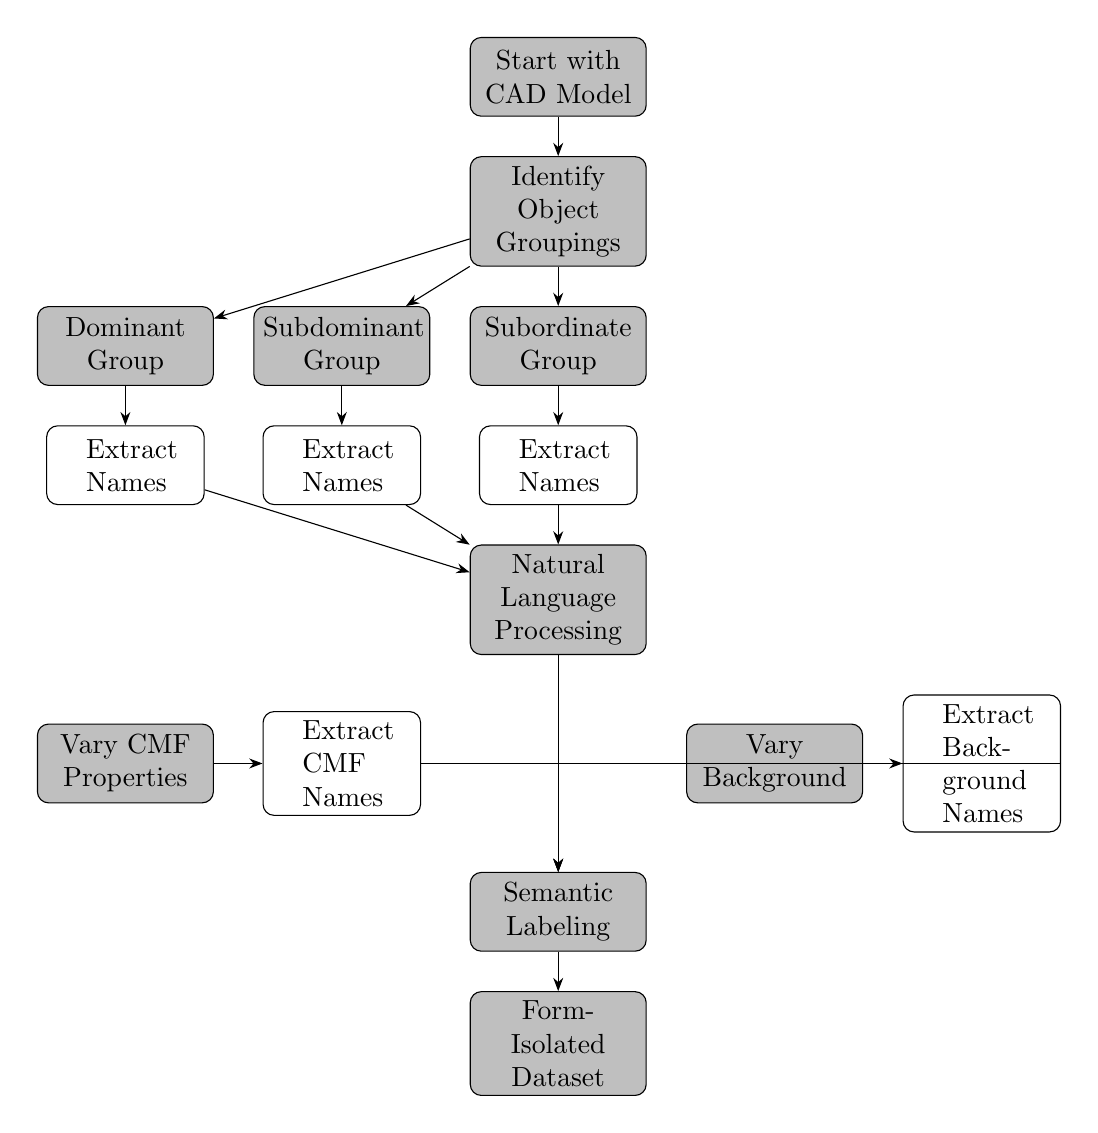
\begin{tikzpicture}[
        block/.style={rectangle, draw, fill=lightgray, rounded corners, minimum width=2cm, minimum height=1cm, align=center, text width=2cm}, % Add text width
        extract/.style={rectangle, draw, fill=white, rounded corners, minimum width=2cm, minimum height=1cm, align=left, text width=1cm}, % Add text width
        arrow/.style={-Stealth},
        matrix of nodes,
        column sep=0.5cm, 
        row sep=0.5cm,    
        nodes={align=center, anchor=center}
      ]

      \matrix (m) {
        & & \node[block] (start) {Start with CAD Model}; & & \\
        & & \node[block] (objectgrouping) {Identify Object Groupings}; & & \\
        \node[block] (dominantgroup) {Dominant Group}; & 
        \node[block] (subdominantgroup) {Subdominant Group}; &
        \node[block] (subordinategroup) {Subordinate Group}; \\
        \node[extract] (extractdominant) {Extract Names}; & 
        \node[extract] (extractsubdominant) {Extract Names}; & 
        \node[extract] (extractsubordinate) {Extract Names}; \\
        & & \node[block] (nlp) {Natural Language Processing}; & & \\
        \node[block] (cmfvariation) {Vary CMF Properties}; & 
        \node[extract] (extractcmf) {Extract CMF Names}; &
        &
        \node[block] (varybackground) {Vary Background}; &
        \node[extract] (extractbackground) {Extract Background Names}; \\
        & & \node[block] (semanticlabeling) {Semantic Labeling}; & & \\
        & & \node[block] (dataset) {Form-Isolated Dataset}; & & \\
      };

      \draw[arrow] (start) -- (objectgrouping);
      \draw[arrow] (objectgrouping) -- (dominantgroup);
      \draw[arrow] (objectgrouping) -- (subdominantgroup);
      \draw[arrow] (objectgrouping) -- (subordinategroup);

      \draw[arrow] (dominantgroup) -- (extractdominant);
      \draw[arrow] (subdominantgroup) -- (extractsubdominant);
      \draw[arrow] (subordinategroup) -- (extractsubordinate);

      \draw[arrow] (extractdominant) -- (nlp);
      \draw[arrow] (extractsubdominant) -- (nlp);
      \draw[arrow] (extractsubordinate) -- (nlp);

      \draw[arrow] (cmfvariation) -- (extractcmf);
      \draw[arrow] (varybackground) -- (extractbackground);

      \draw[arrow] (nlp) -- (semanticlabeling);
      \draw[arrow] (extractcmf.east) -| (semanticlabeling.north); 
      \draw[arrow] (extractbackground.east) -| (semanticlabeling.north); 

      \draw[arrow] (semanticlabeling) -- (dataset);

    \end{tikzpicture}
    \caption{Form Isolation through Systematic Variation and NLP Flowchart}
    \label{fig:firstflowchart}
\end{figure}




Figure \ref{fig:firstflowchart} above outlines the process of the system that is detailed below.

\begin{enumerate}
    \item \textbf{Systematic Variation:} The system automatically generates a diverse set of variations of the CAD model by systematically altering visual properties (color, texture, material), camera viewpoints (angle, position, focal length), lighting conditions (intensity, direction, color temperature), and backgrounds (color, texture, environment). Critically, this variation is performed while meticulously preserving the core design form as a constant element. This form isolation is crucial for preventing overfitting and enabling the AI model to learn the underlying design intent rather than superficial stylistic features.

    \item \textbf{Automated Semantic Labeling:} For each generated variation, the system automatically produces descriptive text labels. These labels capture essential attributes of the image, including object groupings, applied variations, and design intent. These labels facilitate the training of the AI model and enable natural language interaction with the system. 

    \item \textbf{AI Model Fine-tuning:} The generated dataset of images and their corresponding semantic labels is used to fine-tune a pre-trained text-to-image AI model, such as Stable Diffusion, using Low-Rank Adaptation (LoRA). LoRA is an efficient technique that allows the model to adapt to the specific design data while preserving its general capabilities learned from a much larger dataset. 

    \item \textbf{AI-Assisted Design Interface:} The invention provides a user-friendly interface for designers to interact with the trained AI model. Designers can input natural language prompts to generate new renderings, specifying adjustments to CMF properties (Color, Material, Finish) and other visual attributes. The interface also includes advanced features:
        \begin{itemize}
            \item Automated file management
            \item Location-based background integration 
            \item Cost and environmental impact analysis 
            \item Automated RFQ (Request For Quotation) generation
            \item Design callouts
            \item Character continuity management
            \item Dynamic UI sliders
            \item Patent drawing generation
            \item Design analysis feedback
            \item Client annotation tools
            \item Image security features
        \end{itemize}
\end{enumerate}

\section{BRIEF DESCRIPTION OF THE DRAWINGS}
Figures \ref{fig:cad_model_groupings} - \ref{fig:location-based-background} illustrate various aspects of the invention.

\begin{figure}[h]
    \centering
    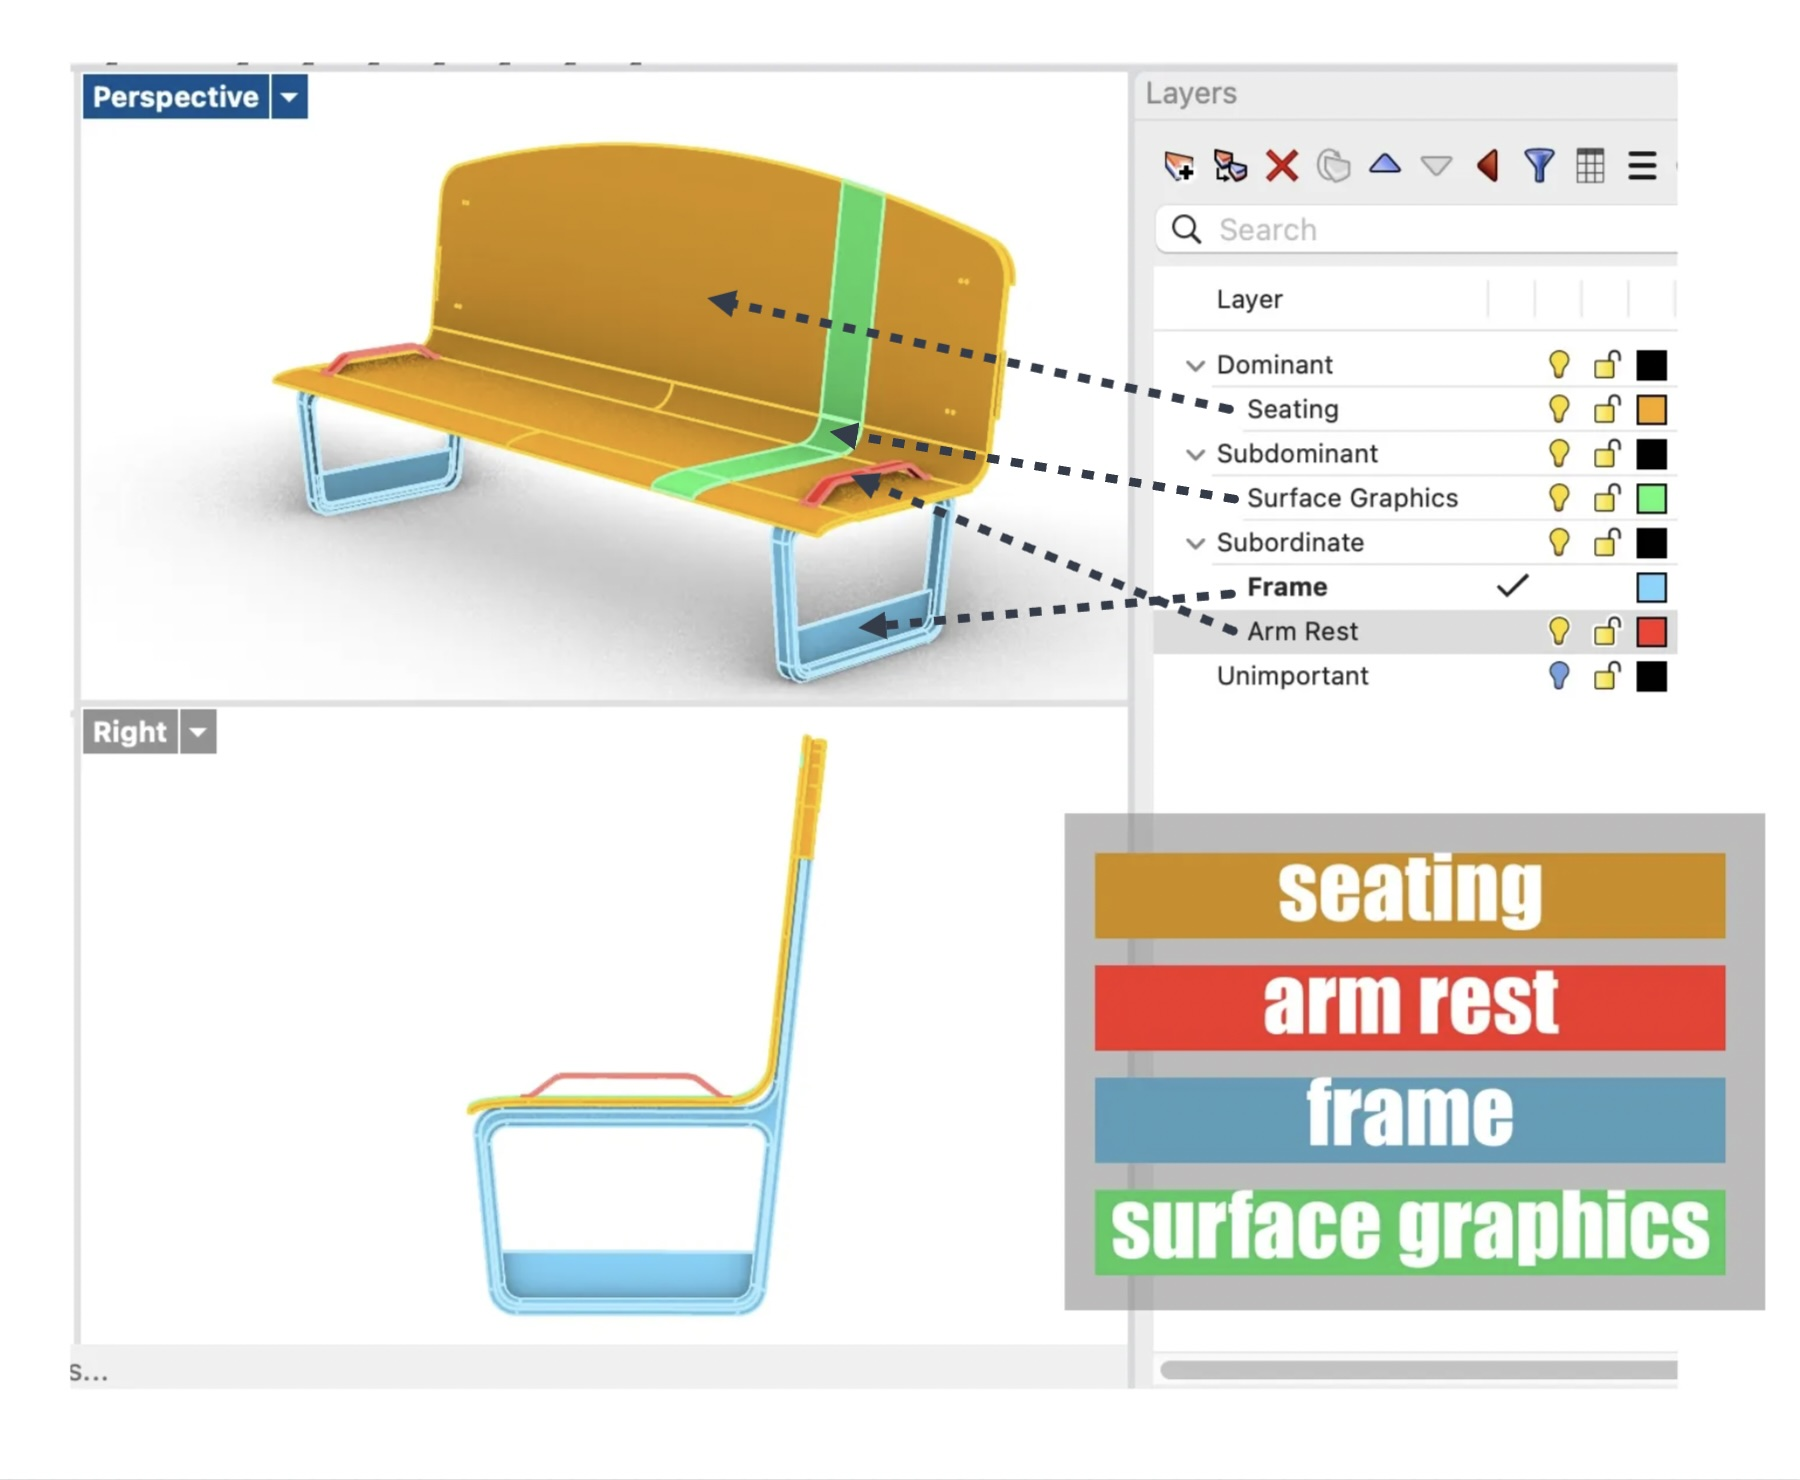
\includegraphics[width=0.8\textwidth]{figures/figure-perspective-right-layers-colors-labled-arrows-2.jpg}
    \caption{CAD Model with Object Groupings and Layer Correspondence}
    \label{fig:cad_model_groupings}
\end{figure}

\begin{figure}[h]
    \centering
    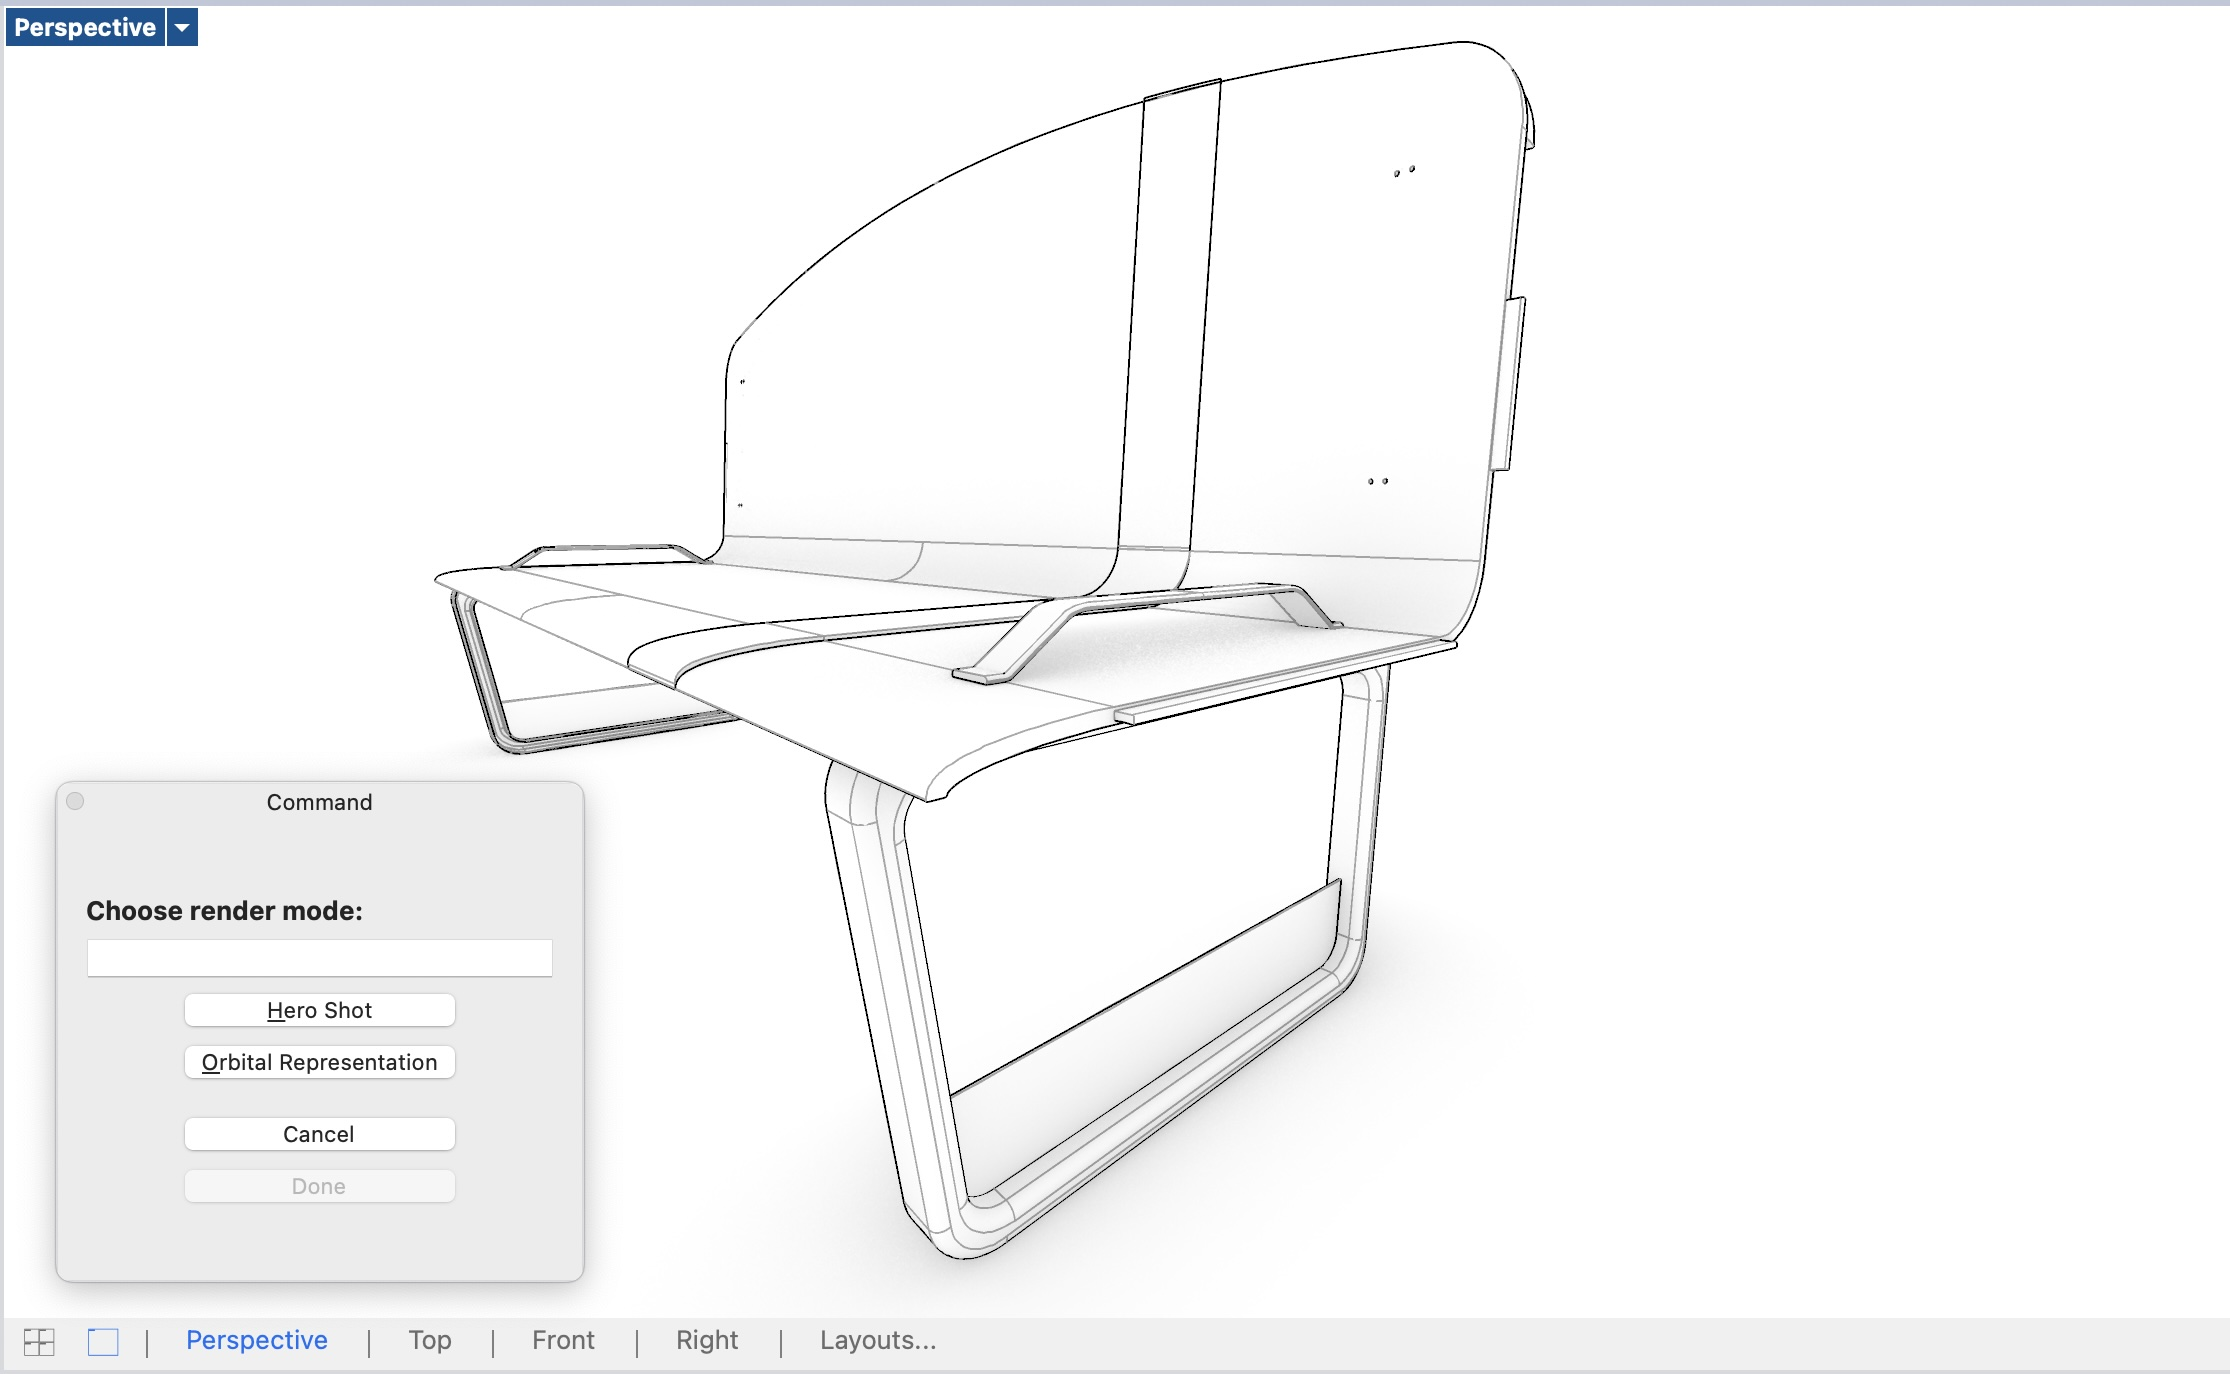
\includegraphics[width=0.8\textwidth]{figures/figure-process-choose-render-mode-monochrome.jpg} 
    \caption{Optionally in some embodiments, selecting the rendering mode of the Training Data Generation Module}
    \label{fig:render_mode_selection}
\end{figure}

\begin{figure}[h]
    \centering
    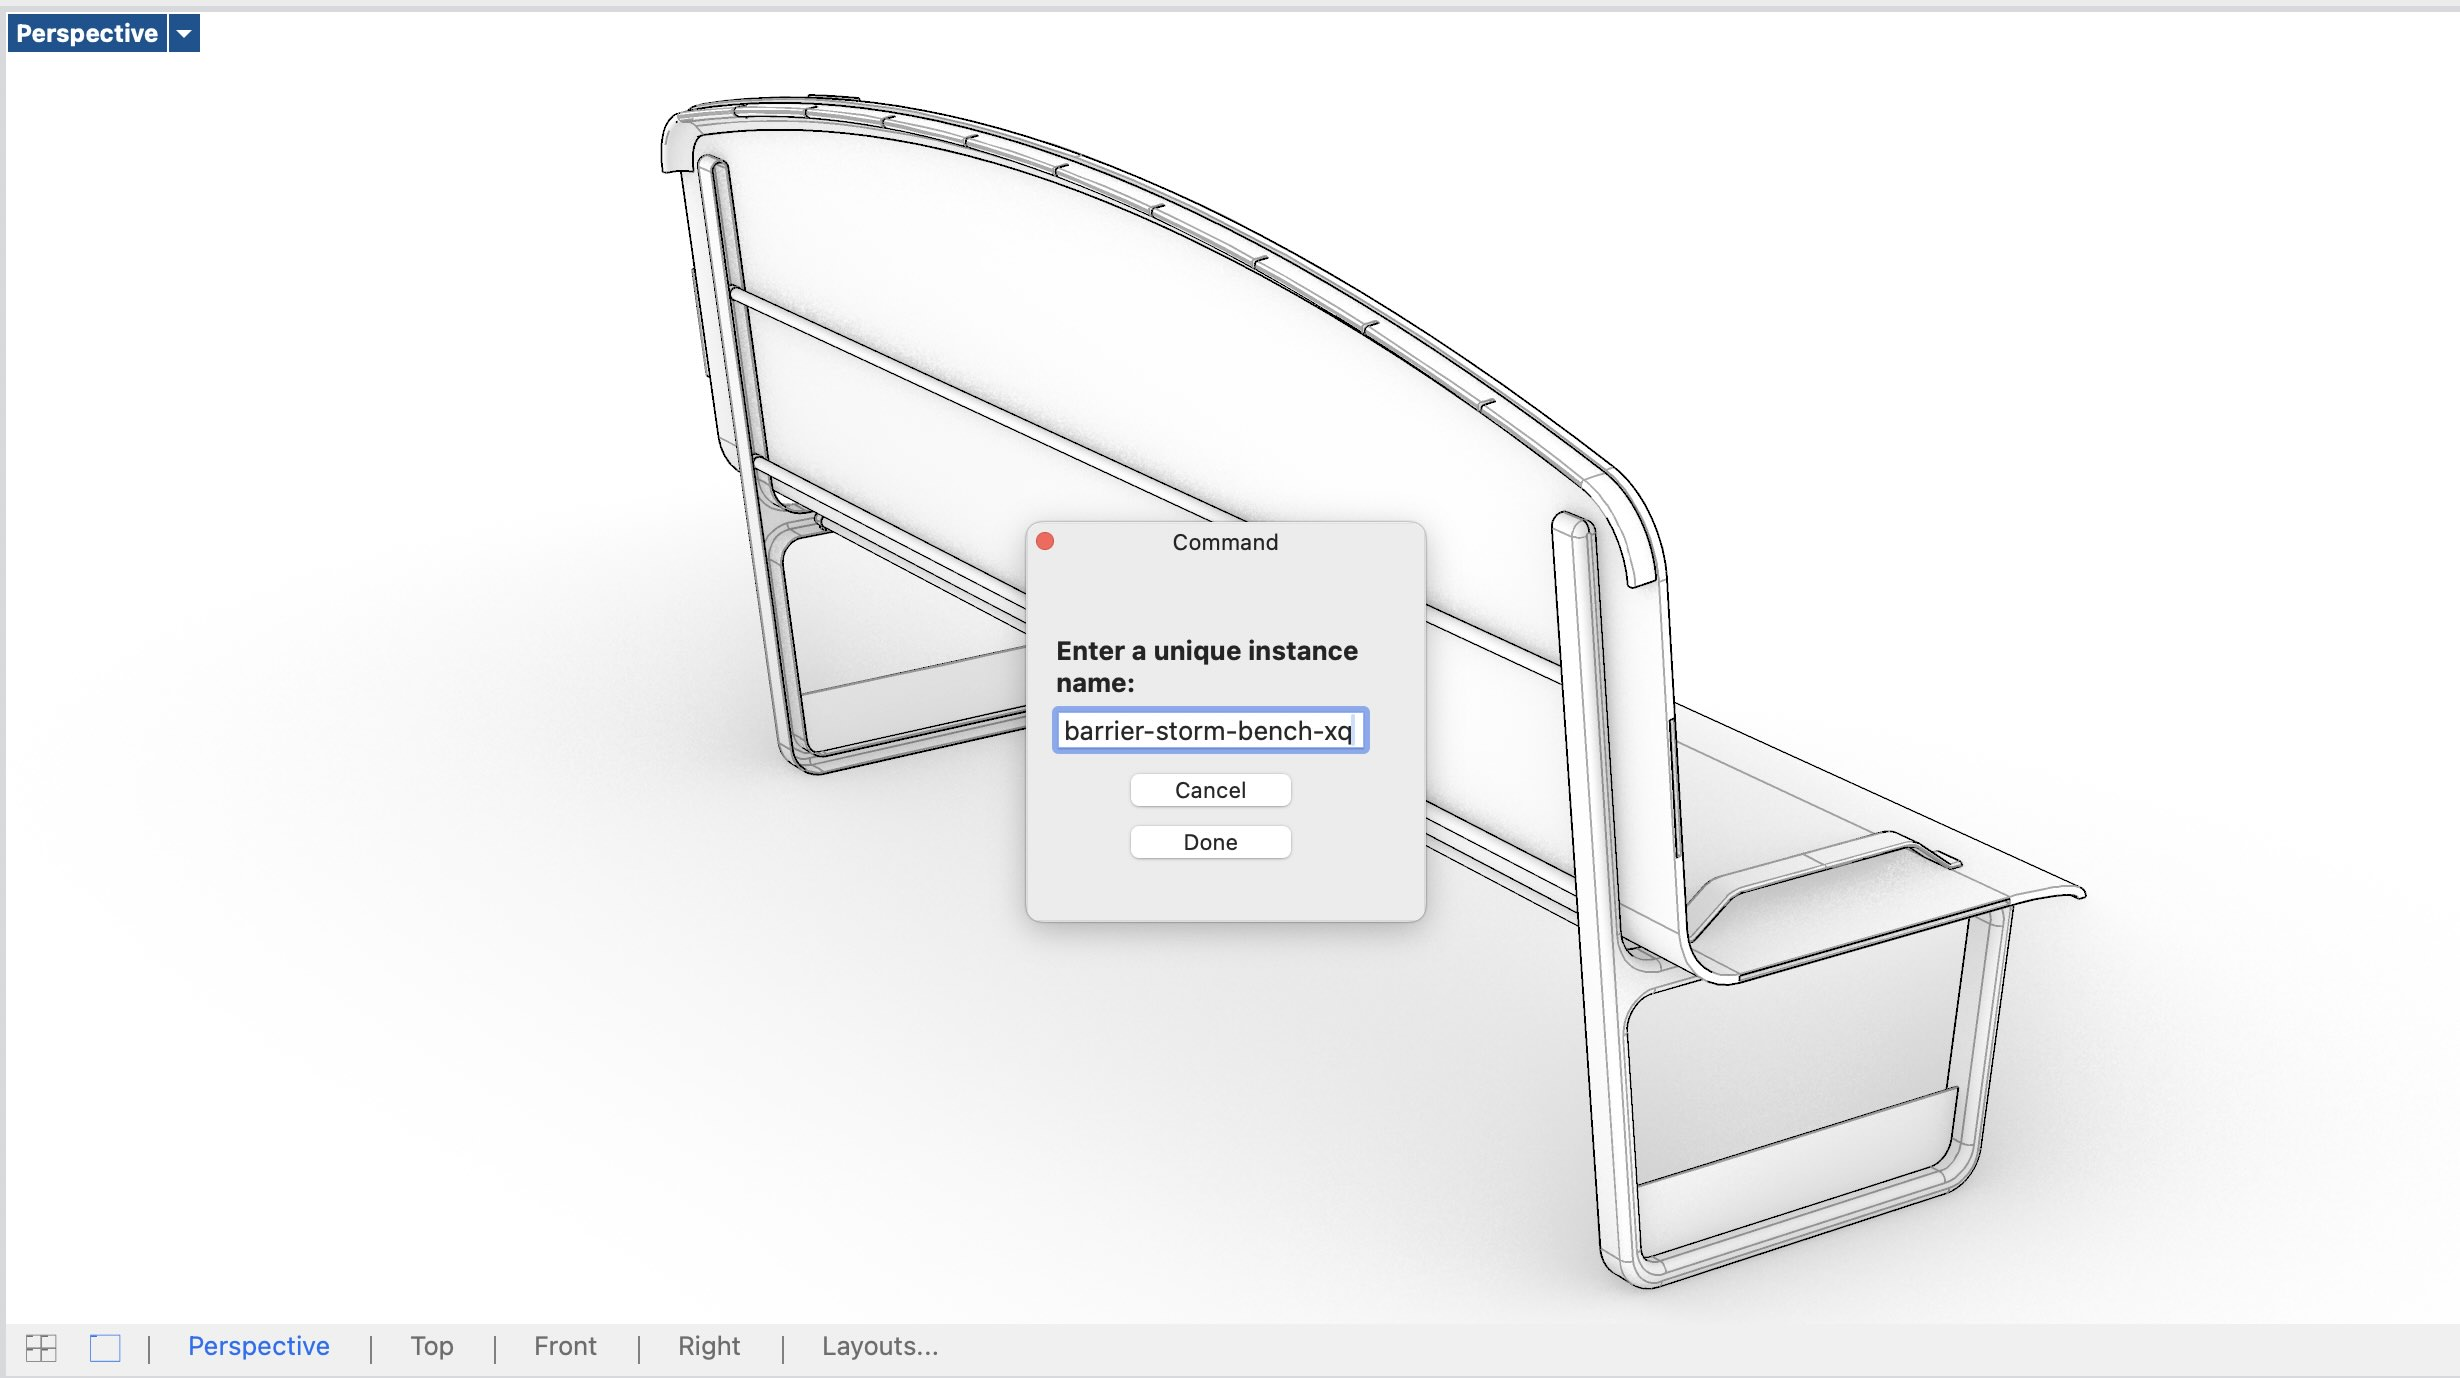
\includegraphics[width=0.8\textwidth]{figures/figure-process-instance-name-barrier-1up-xy-monochrome.jpg}
    \caption{Entering a Unique Instance Name - The user interface prompts the designer to enter a unique instance name for the object being rendered. This instance name, along with other relevant information (class name, lighting, etc.), forms part of the semantic label for each generated variation. These labels provide textual descriptions that help the AI model associate visual features with specific attributes.}
    \label{fig:instance_name_input}
\end{figure}

\begin{figure}[h]
    \centering
    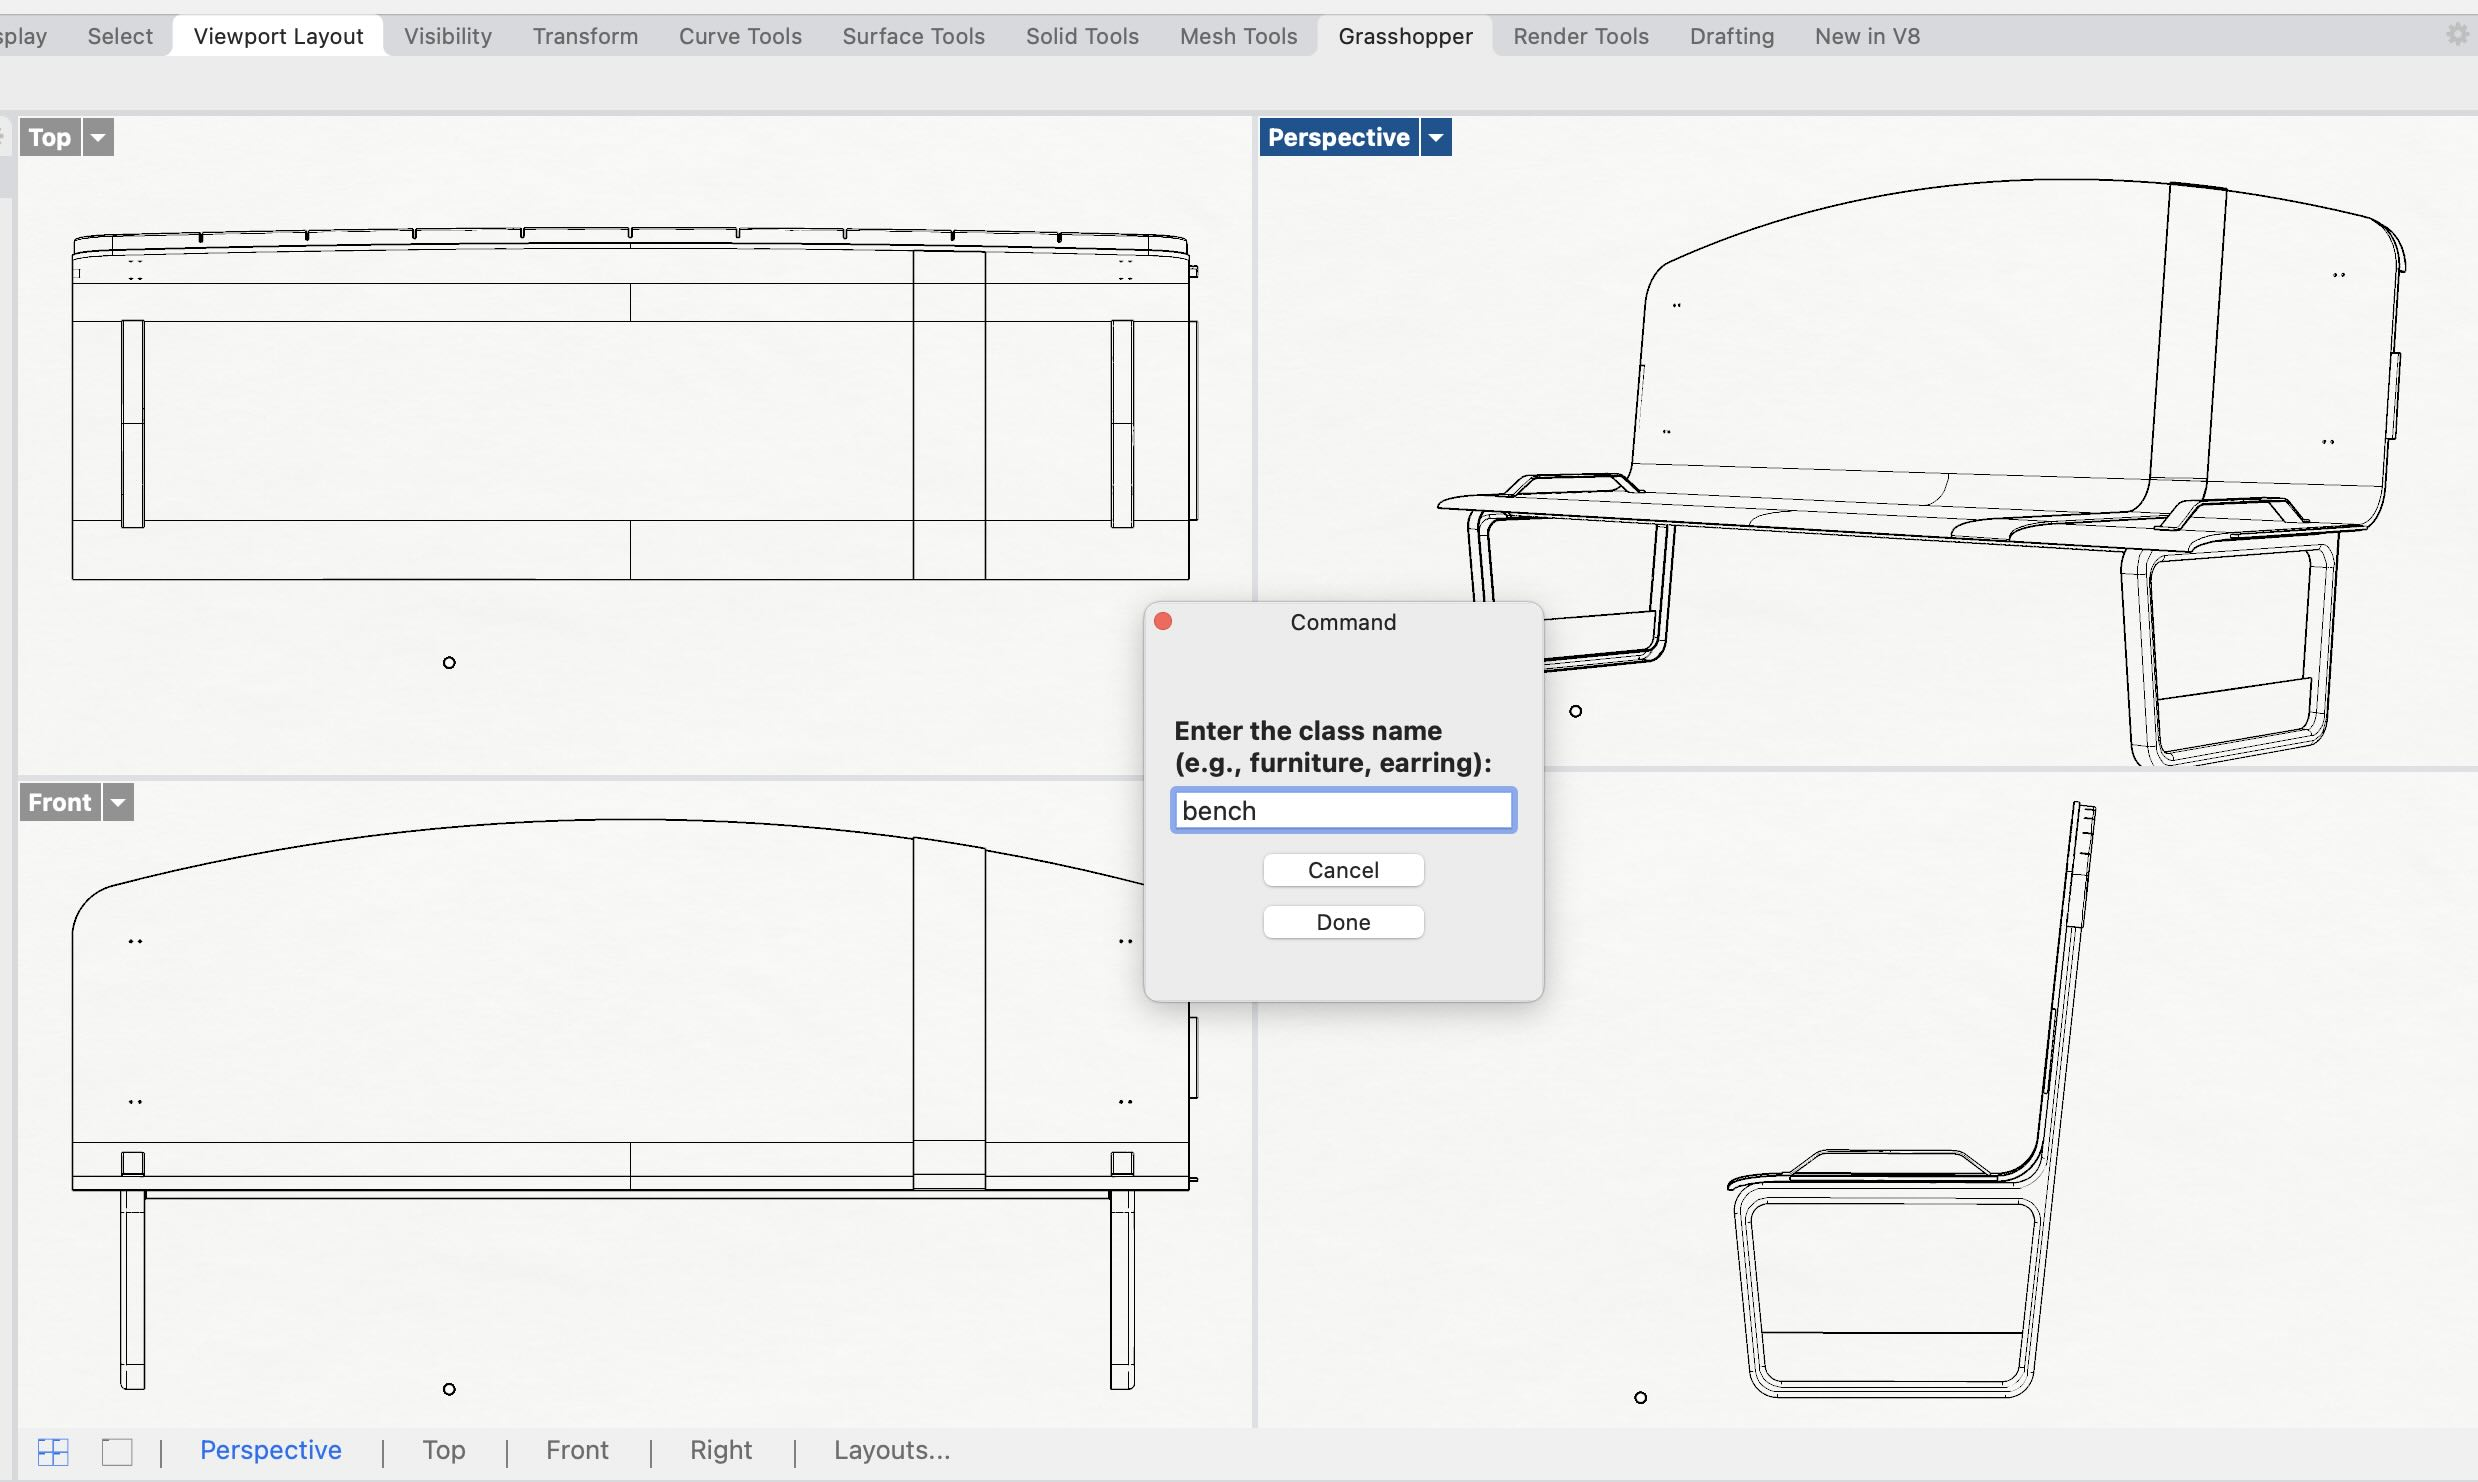
\includegraphics[width=0.8\textwidth]{figures/figure-process-class-name-bench-4up-bw.jpg}
    \caption{Specifying the Class Name - The user interface prompts the designer to enter a class name for the object, providing a broader categorization that helps the AI model understand the object's general type (e.g., furniture, vehicle, appliance). This class name, along with the instance name and other details, forms part of the semantic label for each variation.}
    \label{fig:class_name_input}
\end{figure}

\begin{figure}[h]
    \centering
    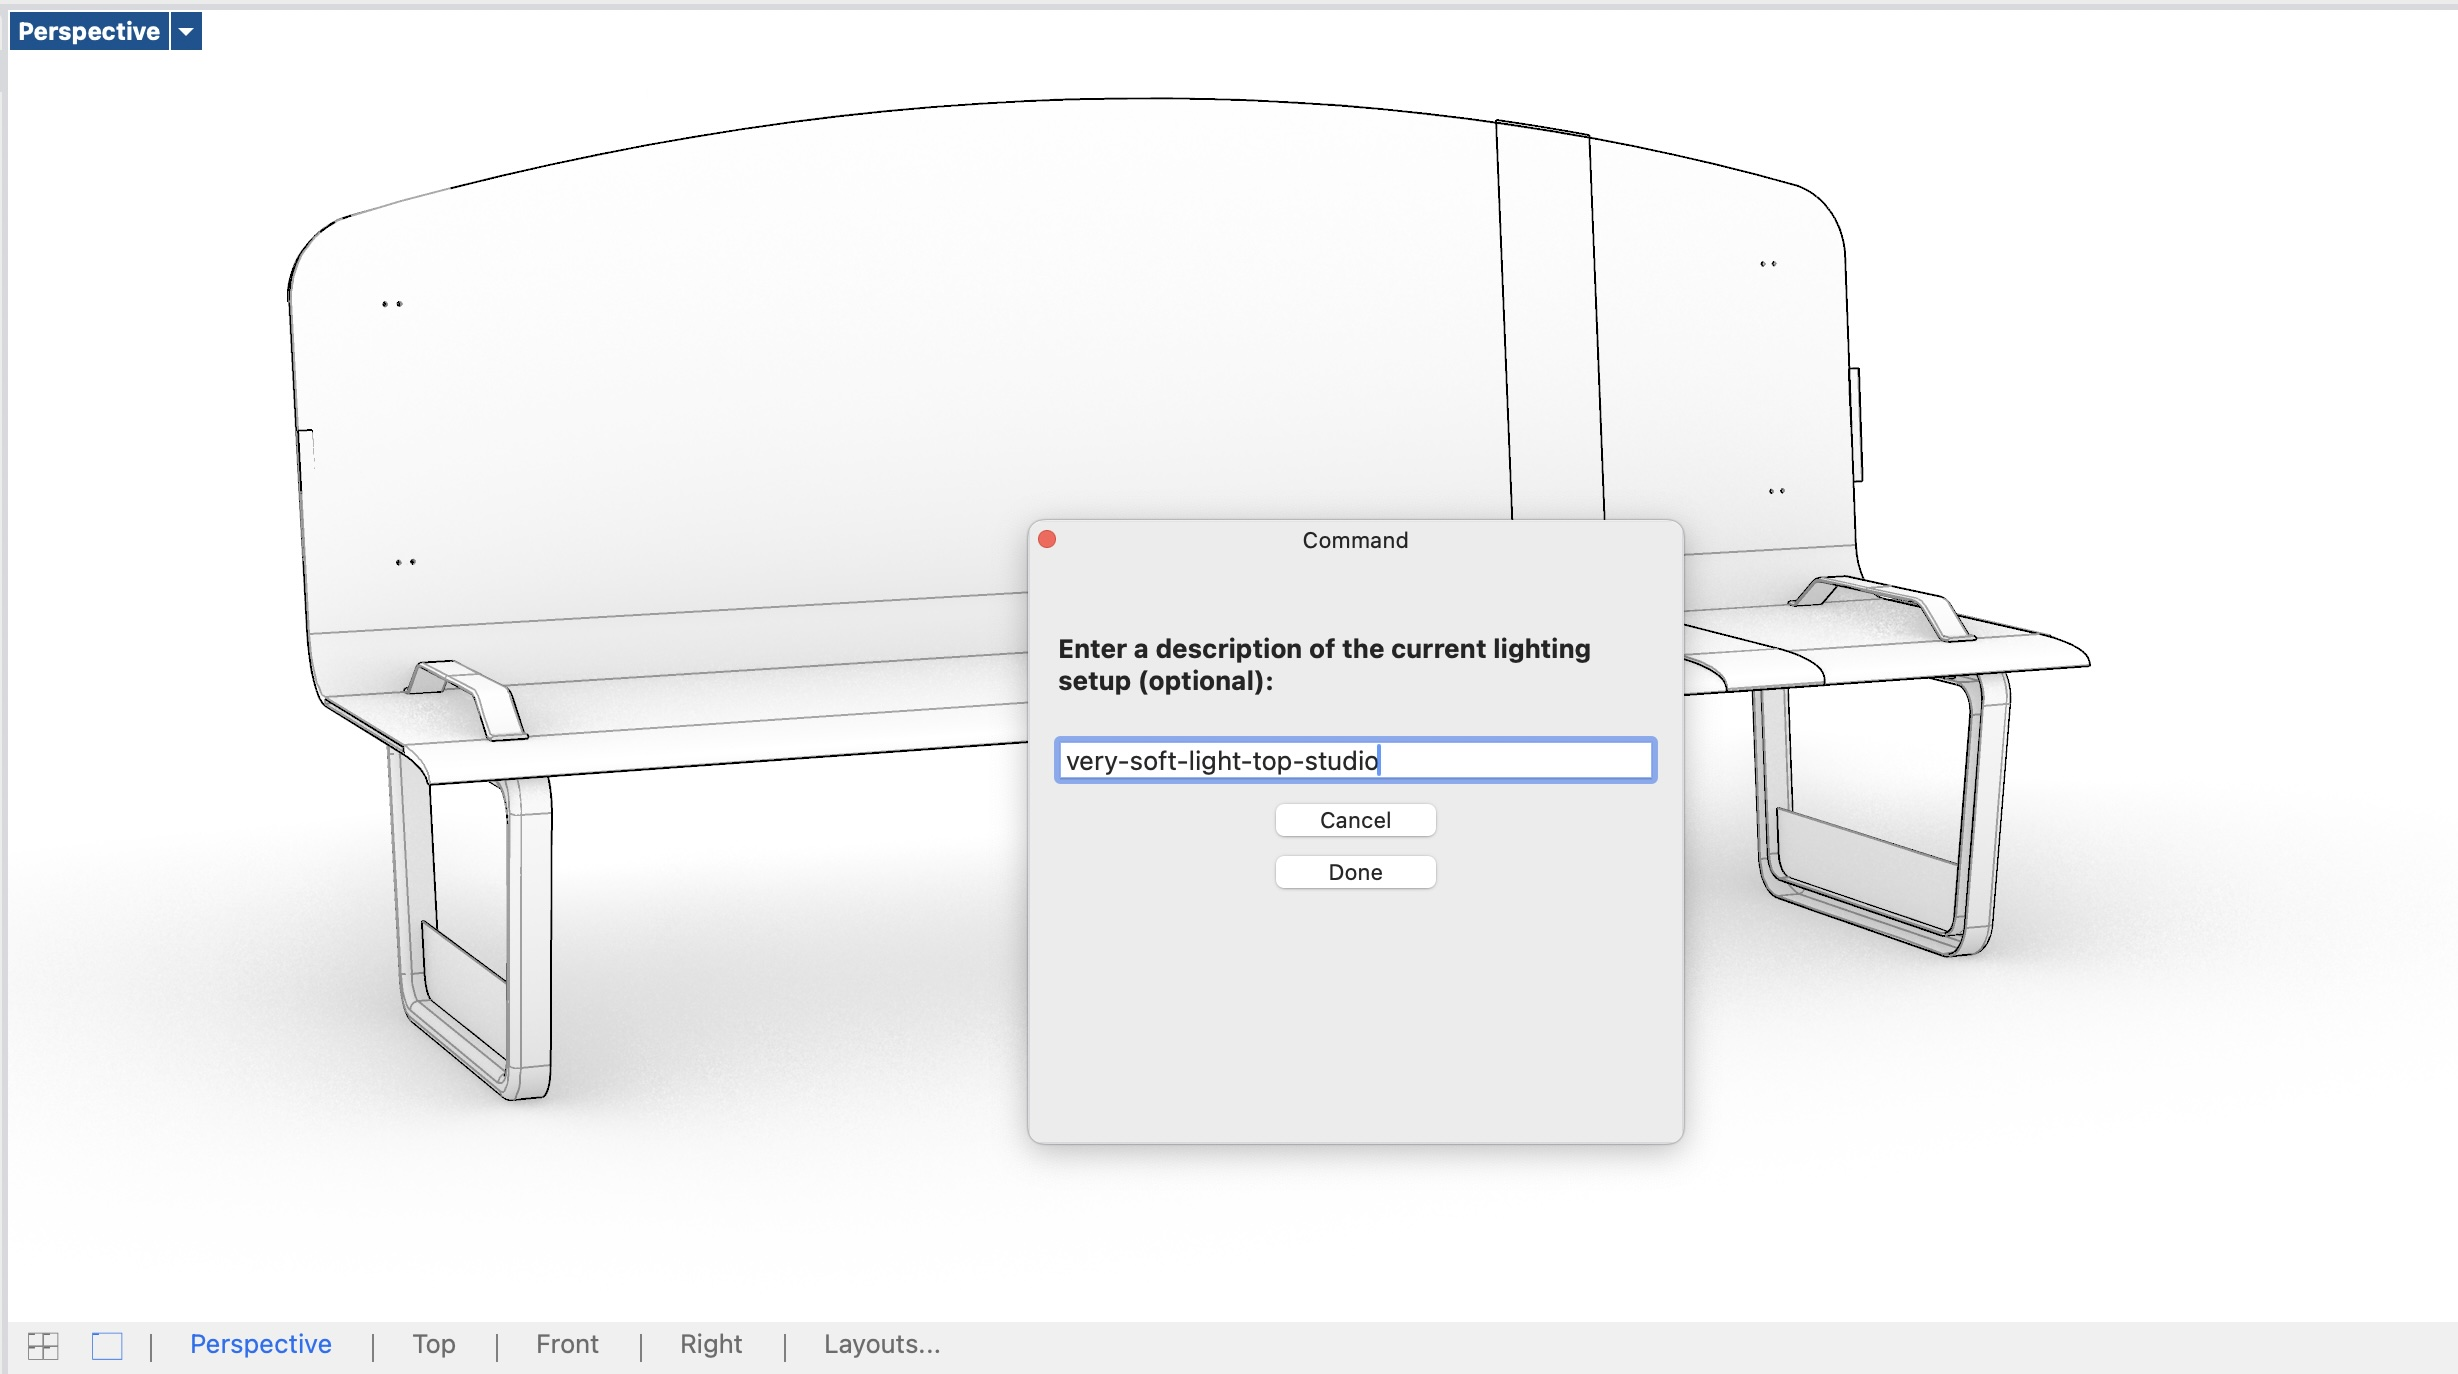
\includegraphics[width=0.8\textwidth]{figures/figure-process-light-description-monochrome.jpg}
    \caption{Describing the Lighting Setup - The user interface allows the designer to enter a description of the lighting setup used for each rendering. This information, captured as part of the semantic label, enables the AI model to learn the relationship between lighting conditions and the object's appearance. In this example, the description "very-soft-light-top-studio" provides a concise representation of the lighting setup.}
    \label{fig:lighting_description_input}
\end{figure}





\begin{itemize}
    \item Figure \ref{fig:cad_model_groupings}: CAD Model with Object Groupings and Layer Correspondence
    \item Figure \ref{fig:render_mode_selection}: User Interface for Variation Setup - Selecting the Rendering Mode
    \item Figure \ref{fig:instance_name_input}: User Interface for Variation Setup - Entering a Unique Instance Name
    \item Figure \ref{fig:class_name_input}: User Interface for Variation Setup - Specifying the Class Name
    \item Figure \ref{fig:lighting_description_input}: User Interface for Variation Setup - Describing the Lighting Setup
    % \item Figure \ref{fig:flowchart}: Form Isolation through Systematic Variation Flowchart
    \item Figure \ref{fig:automated-design-callout}: Automated Design Callout Generation
    \item Figure \ref{fig:modular-ui-texture-style}: Modular User Interface for Texture and Style Application
    \item Figure \ref{fig:location-based-background}: Location-Based Background Integration using Google Maps
\end{itemize}


\section{DETAILED DESCRIPTION OF THE INVENTION}


\subsection{Object Grouping in CAD Models}

The system is designed to be compatible with various industry-standard CAD software, enhancing its accessibility and integration into existing design workflows. While the principles of the invention apply broadly, specific implementations leverage particular features of different CAD packages. The system requires that the CAD software supports modular object organization and provides programmatic access to model data. These features are crucial for automating variation generation and semantic labeling.

\paragraph{Supported Software}
Specifically, the current implementation supports the following CAD software:

\begin{itemize}
    \item \textbf{Rhinoceros 3D (Rhino):} Rhino, with its robust scripting API using Python, enables deep integration with the Automated Data Generation Module. Examples of Rhino and Python code provided herein illustrate this integration. Skilled practitioners can readily adapt these examples to other design software and APIs.
    \item \textbf{Fusion 360:} Fusion 360, widely used in engineering and product design, is a target platform for this invention. Its Python API provides functionalities similar to those in Rhino, allowing seamless integration with the Automated Data Generation Module.
    \item \textbf{SolidWorks:} SolidWorks can be integrated with the system through its API, which can be accessed from Python using COM interop, enabling functionalities similar to those in Rhino and Fusion 360. Alternatively, the system can be adapted to directly utilize the native C++ API of SolidWorks.
\end{itemize}

The core principles of the invention are applicable across different CAD platforms, as long as they offer similar functionalities in terms of object hierarchy and programmatic access.

\paragraph{Object Grouping Mechanisms}

The system is adaptable to different object grouping mechanisms used by various CAD software:

\begin{itemize}
    \item \textbf{Layers (Rhino):} In Rhino, layers (and sublayers) are used for object organization. The provided code illustrates how layer-based groupings correspond to the invention's object grouping concept. For example, different parts of a chair model are grouped into sublayers like  "Chair::Legs," "Chair::Seat," and "Chair::Backrest," allowing for applying material variations based on layer assignment.

    \item \textbf{Components (Fusion 360):} Components in Fusion 360, similar to layers in Rhino, represent distinct parts or sub-assemblies within a design. The system can be adapted to utilize component information for object grouping and variation generation.

    \item \textbf{Groups/Bodies (SolidWorks):} SolidWorks utilizes groups and bodies for organizing geometry. The system can be implemented to recognize these groupings for applying variations and generating semantic labels.
\end{itemize}

Irrespective of the specific CAD software or its internal representation, the core concept of organizing objects hierarchically to represent design intent remains consistent.



\paragraph{Importing and Preprocessing CAD Data}
Importing CAD models and any necessary preprocessing steps are essential for compatibility and efficient data handling.

\subparagraph{Mesh Conversion}

In some cases, conversion of CAD geometry into a mesh representation might be necessary for efficient rendering and processing. The system handles mesh data, maintaining object groupings and applying variations to mesh elements. If mesh conversion is required, the system prioritizes using the highest fidelity mesh representation, balancing detail and computational efficiency.

\subparagraph{Geometry Simplification}
For complex CAD models, geometry simplification techniques, such as mesh decimation or NURBS curve reduction, can be used to reduce computational load during variation generation and rendering. The system incorporates parameters to control the simplification level, allowing designers to balance detail with performance. The system provides feedback to the designer if simplification is necessary and allows for adjustment of simplification parameters.

\subsection{Automated Data Generation Module}

The Automated Data Generation Module is the core of the invention, responsible for creating the diverse and richly labeled dataset required to train the AI model. It interacts directly with the CAD system, extracting object groupings, applying systematic variations, and generating corresponding semantic labels.


\subparagraph{Illustrative Embodiment} 

Here is a simplified example of the code in one exemplary CAD system, Rhino:

\begin{verbatim}
def get_objects_from_sublayers():
"""Get all objects from sublayers, organized by sublayer name."""
sublayers = get_all_sublayers()
objects_by_sublayer = {}
for sublayer in sublayers:
    objects = rs.ObjectsByLayer(sublayer)
    if objects:
        objects_by_sublayer[sublayer] = objects
return objects_by_sublayer

\end{verbatim}  

which would be called in conjunction with 

\begin{verbatim}
def apply_random_materials():

    objects_by_sublayer = get_objects_from_sublayers()
    materials = {}
    
    #Apply varied materials to all object in sublayers.
    for sublayer, objects in objects_by_sublayer.items():
        material_index, material_name = create_random_material()
        
        for obj in objects:
            rs.ObjectMaterialIndex(obj, material_index)
        
        sublayer_name = sublayer.split("::")[-1].lower()
        
        # Create a grammatically correct description
        description = f"{material_name} {sublayer_name}"
        
        materials[sublayer_name] = {
            'name': sublayer_name,
            'material': material_name,
            'description': description
        }
    
    print(f"\nApplied materials: {materials}")
    return materials

\end{verbatim}  

Finally the names of the applied materials are for future labeling purposes:
\begin{verbatim}
def create_readable_material_description(materials):
    """Create a readable description of materials using sublayer names."""
    descriptions = []
    for material_info in materials.values():
        descriptions.append(material_info['description'])
    
    return ", ".join(descriptions)
\end{verbatim}  

Explicit modularity (provided as an example as layer-based grouping in Rhino) allows a direct mapping between the designer's CAD model's organization and the system's understanding of the design components. The system applies predictable variation to the CAD model to encode the most essential properties of design: the form itself.

\paragraph{Object Visual Properties}

\subparagraph{Visual Properties (CMF)}
The system varies the color, material, and finish (CMF) properties of objects within defined groupings, ensuring a diverse range of variations for the training dataset.

% \textbf{Randomness and Predefined Ranges:}

% The code example showcases the use of randomness and predefined ranges for material assignment. For example, a data structure such as \texttt{MATERIAL\_LIST} defines a library of materials with their associated properties (name, RGB color, gloss, and reflectivity). A function with a name such as \texttt{create\_random\_material()} randomly selects a material from this list and applies it to the objects within a group. This randomized set-based approach ensures a diverse range of CMF variations in the training dataset and the accuracy of the semantic labeling.

\subparagraph{Randomness and Predefined Ranges}
 The provided code examples demonstrate how a data structure like \texttt{MATERIAL\_LIST} defines a library of materials with associated properties (name, RGB color, gloss, reflectivity). Functions like \texttt{create\_random\_material} select materials randomly from this library, ensuring diversity in CMF variations.

\begin{verbatim}
MATERIAL_LIST = [
("Soft Red Plastic", (220, 60, 50), 30, 0.2),
("Forest Green Metal", (34, 139, 34), 80, 0.5),
("Navy Blue Fabric", (0, 60, 120), 20, 0.1),
("Mustard Yellow Leather", (225, 173, 1), 40, 0.15),
("Teal Ceramic", (0, 128, 128), 70, 0.2),
("Plum Wood", (142, 69, 133), 50, 0.3),
("Off White Paint", (245, 245, 240), 25, 0.1),
("Charcoal Rubber", (54, 69, 79), 35, 0.05),
...etc...
\end{verbatim}

\paragraph{Camera Viewpoints and Perspectives}
The system varies the camera perspective to capture the design from different angles and distances, enhancing the AI model's understanding of the form.

\subparagraph{Hero Shot and Orbital Representation}
Two examples implemented in Rhino are 'Hero Shot' and 'Orbital Representation.' 'Hero Shot' clusters camera positions around a designer-chosen focal point, simulating product photography. The `variation\_degrees` parameter controls randomness in camera positioning. 'Orbital Representation' places cameras along circular or elliptical paths around the object for comprehensive views. The system can utilize various patterns for camera paths to generate diverse viewpoints. In varying camera perspectives, simulated lens length may also be varied, as well as other aspects such as depth of field, further enriching the dataset and isolating the form.

\paragraph{Lighting}
The system generates diverse lighting scenarios mimicking various environments and times of day. For example, the function `generate\_lighting\_variation` varies lighting parameters like softness, direction, and intensity. It also stores the corresponding natural language descriptions for labeling.

\paragraph{Backgrounds}
The system applies diverse backgrounds to the rendered images, improving context and visual diversity. It uses a library of predefined backgrounds (colors, gradients, textures, scenes). The system also integrates with Google Maps, allowing real-world locations as backgrounds, with accurate placement and perspective using depth maps and ControlNet.

\subsubsection{Semantic Label Generation}
For every variation generated, the system creates a detailed semantic label. The `generate\_caption` function provides an example. Labels include information about:

\begin{itemize}
    \item Object Groupings and Materials
    \item Camera Viewpoint
    \item Lighting Conditions
    \item Background
\end{itemize}

Semantic labels are used in file naming or stored in descrete data structures (e.g., JSON) that linked to the training dataset images. These lables describe the differences between images in the dataset, providing for the AI model's understanding of the relationship between textual descriptions and visual attributes.

\paragraph{Synthetic Augmentation Techniques}

In addition, the system may use data augmentation to increase dataset diversity and model robustness, including:

\begin{itemize}
    \item Random Cropping
    \item Rotation and Flipping (while considering physical interactions and accurate labeling)
    \item Color Jitter
    \item Noise Addition 
\end{itemize}

The specific data augmentation techniques are customizable based on the design context and dataset characteristics.

\subsection{AI Model Training Module}
This module imbues the AI model with the ability to understand and generate variations of the designer's intended form, focusing on the core form independent of stylistic variations.

\subsubsection{Pre-trained Model Selection}
The system uses a pre-trained text-to-image AI model. Key criteria for selection include:
\begin{itemize}
    \item Open-Source License: for control over customization, deployment, and future development.
    \item Architectural Flexibility: adaptability for efficient fine-tuning (e.g., using LoRA).
    \item Adequate Image Quality: sufficient quality and resolution for design visualization purposes.
\end{itemize}
Potential candidates include Stable Diffusion and other emerging diffusion-based models known for their flexibility and efficiency.

\subsubsection{Training for Form Recognition}

The training emphasizes form recognition over stylistic imitation.

\paragraph{Dataset Structure}
The dataset comprises numerous variations of the same design. The form remains constant while visual attributes (CMF, viewpoints, lighting, backgrounds) are varied, directing the AI's focus to the consistent form.

\paragraph{Semantic Label Guidance}
Semantic labels emphasize the underlying form and its constituent parts. They guide the AI to learn a representation of the form decoupled from stylistic variations.


\subsubsection{Fine-tuning with LoRA}
Low-Rank Adaptation (LoRA) is used to fine-tune the pre-trained model efficiently without full retraining.

\paragraph{Benefits of LoRA}
\begin{itemize}
    \item Targeted Modification: LoRA injects small matrices into specific layers, enabling targeted adjustments without disrupting general capabilities.
    \item Preventing Overfitting: LoRA's efficiency reduces the risk of overfitting to specific variations in the form-focused dataset.
\end{itemize}

Multiple LoRAs can be used in combination, allowing simultaneous rendering of multiple unique objects in a scene.

\subsubsection{Evaluation and Validation}
The training process is monitored and evaluated to ensure the model's effectiveness.

\begin{itemize}
    \item Visual Inspection: Designers assess generated images for fidelity to the original form.
    \item Quantitative Metrics: Metrics like FID and CLIP Score can be used, but interpreted in the context of form representation rather than photorealism.
    \item Generalization Tests: Testing on unseen prompts and variations ensures the AI can generalize and generate novel variations while preserving design characteristics.
\end{itemize}

\subsection{AI-Assisted Design Interface}
This user-friendly interface bridges the designer's intent and the AI's rendering capabilities.

\subsubsection{Core Rendering Functionality}

\paragraph{Natural Language Prompts}
Designers interact using natural language descriptions for CMF changes, lighting adjustments, viewpoints, and scene elements.

\paragraph{Prompt Parsing and Parameter Translation}
The interface parses prompts using natural language processing, identifying key elements and translating them into rendering parameters for the AI model. This includes:

\begin{itemize}
    \item Object References: using object groupings from the CAD model.
    \item CMF Properties: extracting desired changes to color, material, and finish.
    \item Lighting and Viewpoint: interpreting descriptions for lighting conditions and camera viewpoints.
\end{itemize}

\paragraph{Rendering Generation}
Guided by the extracted parameters, the AI model generates renderings while preserving the integrity of the original form, allowing for manipulation of visual attributes without altering the fundamental design.

\subsubsection{Advanced Features}
The interface offers a suite of advanced features:

\paragraph{Automated File Management}

\begin{itemize}
    \item Automated Naming: generates descriptive file names based on prompt content.
    \item Cloud Storage: automatically stores renderings and associated data in the cloud with version control.
    \item Archiving: facilitates project archiving for easy retrieval.
\end{itemize}


\subsubsection{Details and Close-Ups}
\begin{itemize} 
    \item Designers can specify regions of interest within the prompt or directly on the rendered image to generate high-resolution close-ups of specific design elements. For instance, a prompt could include "generate a detailed close-up of the joinery details on the armrest." Provided "joinery" was modularized in the pre-training phase -- for example, grouped, named, and assigned to the subordinate layer -- explicit manipulation is generally possible via natural language.
\end{itemize} 


\subsubsection{Location-Based Backgrounds}
\begin{itemize}
\item \textbf{Google Maps Integration}: The system seamlessly integrates with Google Maps, allowing designers to select real-world locations as backgrounds for their renderings. The user can specify a location and viewpoint directly within the prompt (e.g., "place the bench in Central Park, facing the Bethesda Terrace," as depicted in Figure \ref{fig:location-based-background}).

\item \textbf{Depth Map Generation}: The system automatically retrieves depth information from Google Maps data for the chosen location. This depth data is used to create a 3D representation of the environment, which is employed by ControlNet such that the description of the scene elements (central park, New York City Skyline) match the actual contours of the buildings from a particular perspective, which is currently beyond the capabilities of generative AI unaided in this manner. Because the AI understands the essential form of the object and its status, relative to the gravity vector and its class and thus relationship to the world, no manual manipulation of its relationships between the design. This allows the object and the background to be rendered within a realistic background context without tedious manipulation of focal length, perspective, and object placement. It just looks right.
\end{itemize}

\begin{figure}[h]
    \centering
    \includegraphics[width=1\textwidth]{figures/figure-location-based-background.jpg}
    \caption{Location-Based Background Integration using Google Maps}
    \label{fig:location-based-background}
\end{figure}


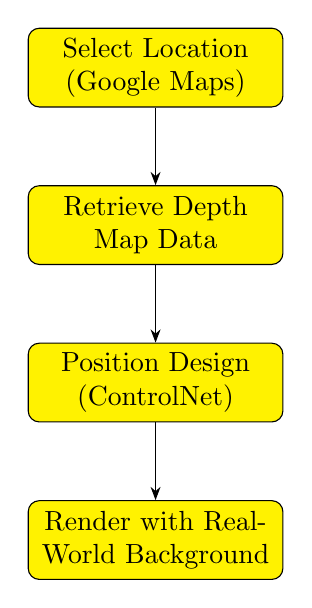
\begin{tikzpicture}[
    node distance=2cm,
    block/.style={rectangle, draw, fill=yellow, rounded corners, minimum width=3cm, minimum height=1cm, text width=3cm, align=center},
    arrow/.style={-Stealth}
  ]

  \node[block] (selectlocation) {Select Location (Google Maps)};
  \node[block, below of=selectlocation] (depthmap) {Retrieve Depth Map Data};
  \node[block, below of=depthmap] (controlnet) {Position Design (ControlNet)};
  \node[block, below of=controlnet] (rendering) {Render with Real-World Background};

  \draw[arrow] (selectlocation) -- (depthmap);
  \draw[arrow] (depthmap) -- (controlnet);
  \draw[arrow] (controlnet) -- (rendering);

\end{tikzpicture}




\subsubsection{Mass \& Volume Calculations}
\begin{itemize}
\item \textbf{Automated Analysis}: Based on the dimensional information from the CAD model and CMF properties extracted from prompt language, the system automatically calculates the estimated weight, volume, and material costs of the design. For example, if the prompt specifies "brushed stainless steel" for a bench frame, the system will calculate the volume of the frame, reference the density of stainless steel, and then calculate the estimated weight and cost based on current market prices.
\item \textbf{Environmental Impact}: The system estimates the environmental impact of the design based on the chosen materials and manufacturing processes. This could involve calculating the carbon footprint based on material extraction, processing, and transportation data. 
\item \textbf{Automated RFQ Generation}: The system can automatically generate requests for quotations (RFQs) based on the calculated material requirements and manufacturing specifications. This could involve automatically filling out web forms or generating emails pre-populated with the relevant design and material information, streamlining the process of obtaining quotes from suppliers.
\end{itemize}

\subsubsection{Design Callouts}
\begin{itemize}
    \item \textbf{Automated Callout Generation}: generates professional-style callouts on rendered images using image segmentation, highlighting relevant design elements and providing annotations based on prompts or rules. 
    \item \textbf{Editable Annotations}: allows designers to edit callout text, positioning, and style.
    \item \textbf{Searchable PDF Export}: embeds callouts as searchable text elements in PDF exports.
    \item \textbf{Consistent Character Appearance}: ensures consistent character appearance across variations.
    \item \textbf{Face Swapping}: employs face-swapping for consistent facial appearance even with variations in other aspects.
    \item \textbf{Text-Based Description Matching}: matches character appearance to designer descriptions from the prompts.
\end{itemize}

\begin{figure}[h]
    \centering
    \includegraphics[width=0.8\textwidth]{figures/figure-automated-design-callout.jpg}
    \caption{Automated Design Callout Generation}
    \label{fig:automated-design-callout}
\end{figure}

\subsubsection{Dynamic UI Sliders}

This feature provides an advanced level of interactivity and control within the AI-assisted design interface, allowing designers to fine-tune rendering parameters intuitively.

\begin{itemize}
    \item \textbf{Context-Sensitive Sliders}: The interface dynamically generates sliders for controlling rendering parameters based on the context of the text prompt. For instance, if a designer inputs a prompt like "a bench against a backdrop of a stormy sky and waves," the system recognizes elements such as "stormy sky" and "waves." It then generates sliders corresponding to these elements, such as:

    \begin{itemize}
        \item \textbf{Intensity of the Storm}: Adjusts the severity and visual impact of the stormy sky.
        \item \textbf{Turbulence of the Waves}: Controls the roughness or calmness of the water.
        \item \textbf{Brightness of the Lightning}: Modifies the prominence and luminosity of lightning effects.
        \item \textbf{Time of Day}: Alters the overall lighting and atmosphere, from dawn to dusk. In some versions, sliders may be radial, such as to mimic a clock, or take other forms. The point is to convert the language of the designer's rendering prompt and convert that into adjustable sliders to provide fine-grain, quantitative control over the natural language-specified aspects of the environment and CMF.
    \end{itemize}

    \item \textbf{Intuitive Control}: These sliders offer a visual and interactive means for designers to adjust parameters without modifying the text prompt directly. This capability allows for:

    \begin{itemize}
        \item \textbf{Granular Exploration}: Designers can incrementally adjust parameters to observe subtle changes in real-time.
        \item \textbf{Rapid Experimentation}: Facilitates quick iteration by enabling immediate visual feedback from slider adjustments.
        \item \textbf{Enhanced Creativity}: Encourages designers to explore a wider range of design variations that they might not have considered through text prompts alone.
    \end{itemize}

    \item \textbf{Parameter Mapping}: The system intelligently maps slider values to the AI model's rendering parameters:

    \begin{itemize}
        \item \textbf{Adaptive Mapping}: Depending on the parameter's complexity, the mapping can be linear, non-linear, or based on a learned function that correlates slider positions with visual outcomes.
        \item \textbf{Real-Time Rendering}: Even before the sliders are adjusted, the AI model can cache segmented renders as 2D layers whose opacity or blendings are then easily controlled in real-time or near-real-time, providing immediate visual feedback.
        \item \textbf{User Customization}: Designers can customize the range and sensitivity of sliders, tailoring the interface to their specific needs and preferences.
    \end{itemize}

    \item \textbf{Integration with Other Features}: The dynamic sliders work in conjunction with other interface elements:

    \begin{itemize}
        \item \textbf{Preset Management}: Slider configurations can be saved as presets for future use or sharing with team members.
        \item \textbf{Modular UI}: Sliders are part of the modular user interface, allowing designers to add or remove them based on the design context.
        \item \textbf{Design Analysis Feedback}: Adjustments made via sliders can be analyzed by the system to provide feedback or suggestions, enhancing the iterative design process.
    \end{itemize}
\end{itemize}

\textbf{Illustrative Example}:

Consider a scenario where a designer is creating a rendering of a bench designed to withstand storm surges. To create a dramatic rendering, they might write:
\paragraph{}
\texttt{"A dramatic nighttime shot of a partially submerged barrier-storm-bench-xq bench amidst the violent, stormy waters of a hurricane ravaging New York City. The bench, featuring striking orange surface graphics on a weathered dark frame, juts out from the swirling floodwaters, anchored to a submerged walkway. Above, a dark, chaotic sky flashes with lightning, illuminating the city skyline in the distance. Clinging to the bench, a drenched man in a dark shirt and another in a dark polo shirt, both looking weary, try to maintain their grip. Their faces are momentarily lit by flashes of lightning as they brace against the storm. Debris and flotsam—-a submerged park bench, tires-—drift chaotically in the water around them, heightening the sense of catastrophe." }
\paragraph{}
Note the use of the class name \texttt{"bench"} and their instance name \texttt{"barrier-storm-bench-xq"} which invokes the item trained earlier. In some embodiments of the invention, the instance term is inserted into the prompt automatically. To illustrate the functionality of the system, it is written transparently into the prompt.

Based on this prompt, the system generates sliders for:

\begin{itemize}
    \item \textbf{Hurricane Intensity}: Controls the severity of the storm, impacting the waves, wind, and rain.
    \item \textbf{Water Level}: Adjusts how submerged the bench and surrounding environment are.
    \item \textbf{Water Clarity}: Modifies the murkiness or transparency of the water.
    \item \textbf{Lightning Intensity}: Controls the frequency and brightness of lightning strikes.
    \item \textbf{Bench Wear Level}: Adjusts the level of weathering and damage on the bench itself.
    \item \textbf{Surface Graphics Vibrancy}: Modifies the intensity of the orange graphics on the bench.
    \item \textbf{Character Wetness}: Controls how wet the characters on the bench appear.
    \item \textbf{Clothing Tatteredness}: Adjusts the level of tearing and damage to the characters' clothing.
\end{itemize}

By adjusting these sliders, the designer can fine-tune the rendering to achieve the exact visual effect they desire, such as increasing the storm's intensity or making the characters appear more soaked and battered, all without changing the text prompt.

\begin{figure}[H]
    \centering
    \includegraphics[width=0.8\textwidth]{figures/huricane-bench-with-ui.jpg}
    \caption{Fine-tuning a hurricane scene with AI. Sliders control elements like water clarity, bench wear, and clothing tatteredness, enabling precise artistic direction within generated imagery.}
    \label{fig:modular-ui-texture-style}
\end{figure}










\begin{itemize}


\item \textbf{Annotation Placement}: Annotations such as dimension lines, reference numerals, and technical labels are automatically placed according to patent drawing conventions. The system uses the structured data from the CAD model to accurately determine dimensions and relationships between design elements, ensuring that the annotations are placed correctly and comply with patent regulations.

\end{itemize}


\subsubsection{Design Analysis}
\begin{itemize}
\item \textbf{Feedback on environmental context}: The system integrates with a large language model (LLM) like GPT-r or a fine-tuned or specialized LLM. The CMF choices of the designer and the environment are combined with existing logic and natural language processing to produce a prompt that asks an LLM to interrogate potential issues that arise from the new context of the object in its pictured environment. For example, if the prompt specifies "a park bench made of unfinished hickory wood in West Virginia," the LLM could access external knowledgebases to determine that hickory is susceptible to carpenter ant infestations in that region, flagging a potential durability issue. A similar issue could be raised around material suitability with regards to corrosion if a designer specified an enamel painted low carbon steel for a seaside bench near salt spray. This feedback can be presented as text-based warnings, questions. Integration options for commercial suppliers of coatings and finishing are present, for example, recommending a durable two-part epoxy coating for a part that will be exposed to electrolytic solvents such as saltwater, or advertising a new clear coat if the designer specifies "ultra-high gloss" in their natural language CMF prompt. For vendors with products integrated into the system, visual highlights on the rendered image, or even suggested modifications to the design or materials. LoRAs can be created for vendors to enter their coatings into the system (real-world pictures modifying form and environments extensively but keeping the coating the same.) This allows us to all but promise that the industrial design object, once painted with 'rustoleum red,' will look like the picture of 'rustoleum red.'

\item \textbf{Contextual Feedback}: The design analysis takes into account the specific context described in the prompt. For example, if the prompt mentions "outdoor furniture," the LLM might check for weather resistance and UV degradation of the chosen materials. The more context the designer provides in the prompt, the more refined and relevant the design analysis feedback will be.
\end{itemize}

\paragraph{Client Annotation Tools}

\begin{itemize}
    \item \textbf{Collaborative Review}: Allows clients and reviewers to add annotations and feedback directly on rendered images.
    \item \textbf{Visual Feedback}: Enables clients to provide visual feedback through drawing, highlighting, and text boxes.
    \item \textbf{Revision Tracking}: Tracks all annotations and comments for clear record-keeping and iterative revisions.
\end{itemize}


\subsubsection{Image Security}
\begin{itemize}
\item \textbf{Watermarking}: Invisible watermarks are embedded within generated images to protect the designer's intellectual property. These watermarks can contain information about the designer, the project, or the date of creation and can be used to track the origin of the image if it is distributed without authorization.
\item \textbf{Serialization}: Each rendered image is assigned a unique serial number that can be used to track its usage and distribution. This serial number can be linked to specific client information, allowing the designer to monitor who has access to which images.
\item \textbf{Usage Monitoring}: The system can detect if a watermarked image is used without authorization or if it appears in unauthorized locations online. This monitoring could be automated using image recognition techniques and web crawling tools, providing alerts to the designer if unauthorized use is detected.
\end{itemize}

\subsubsection{Vision Tracking \& Form Review}
\begin{itemize}
\item \textbf{Eye-Tracking Integration}: The system can optionally integrate with eye-tracking technology, using the embedded webcam on a laptop or the rear-facing camera on a mobile phone, for example, to analyze user gaze patterns during the review process.
\item \textbf{Heatmap Visualization}: Eye-tracking data is visualized as heatmaps overlaid on the rendered images for the designer to review. The heatmap can indicate which parts of the design are calling the viewer's attention. The degree to which the viewer's attention aligns with the intended hierarchy of design elements can be quantified, providing valuable insights to the designer. It allows for an objective assessment of whether the viewer is noticing the intended focal points of the design or if their attention is drawn to unintended areas. This feedback can guide the designer in refining the composition, proportions, repetition, and contrast of the design elements to achieve the desired visual impact.
\end{itemize}

\subsubsection{Modular UI}
\begin{itemize}
\item \textbf{Drag-and-Drop Interface}: Designers can drag and drop images or textures onto the design to apply materials or patterns, creating a more intuitive and direct way of customizing the rendering. For example, a designer could drag an image of a specific wood grain onto the bench seat to apply that texture, or drag a color swatch from a palette onto the legs to change their color.

\begin{figure}[h]
    \centering
    \includegraphics[width=0.8\textwidth]{figures/figure-modular-ui-texture-style.jpg}
    \caption{Modular User Interface for Texture and Style Application}
    \label{fig:modular-ui-texture-style}
\end{figure}

\item \textbf{Texture Blending}: The system supports blending multiple textures together to create more complex and nuanced material effects. For instance, a designer could blend a rough stone texture with a polished metal overlay to create a unique surface finish, allowing for a greater degree of creative control over the material appearance.
\end{itemize}

\subsubsection{Style References}
\begin{itemize}
\item \textbf{Style Transfer}: Designers can apply different artistic styles to renderings by providing reference images. For example, dragging and dropping a still frame from a Pixar movie could instruct the system to render the design in a similar style, even if the prompt describes realistic materials. This allows designers to explore a wide range of aesthetics beyond photorealism.
\item \textbf{Example of Dynamic Slider Generation}: Sliders control the strength and intensity of the applied style. This allows for fine-grained control over the style transfer effect, enabling the designer to blend the reference style with the original rendering to achieve the desired look. For example, if "low-poly" were used, the prompt interpretation engine might return a "blockiness" slider, or a "mesh detail" slider, as well as a "cartoonyness" slider, whose adjustment, as an example, might lead to exaggeration or understatement of the relative size of the eyes relative to the head; the size of the head relative to the body, or any other aspects associated with "cartoonyness" in the base model. 
\end{itemize}


\paragraph{Preset Management}

\begin{itemize}
    \item \textbf{Saving and Loading Presets}: Allows saving and loading preferred rendering configurations for reuse.
    \item \textbf{Sharing Presets}: Enables sharing presets for consistency and collaboration.
\end{itemize}

\subsubsection{Export Options}
\begin{itemize}
\item \textbf{Image Formats}: The system supports exporting renders in various image formats, including JPG, PNG, TIFF, and EXR, catering to different resolution and quality requirements. This flexibility ensures compatibility with a wide range of design workflows and presentation formats.
\item \textbf{3D Printable Models}: Utilizing a virtual photogrammetry technique, LLM transformer-based technology, or another method, the system can generate a fully textured file ready for printing on a multi-material printer that allows multi-color mixing. A plugin could allow the enablement of a service wherein designers order their 3D printed mockup directly from the interface.


\begin{itemize}
    \item \textbf{Iteration Tracking}: Maintains a history of design iterations, visualized as a tree or timeline.
    \item \textbf{Visual Diff}: Highlights differences between selected versions, aiding iterative refinement.
\end{itemize}

\section{CLAIMS}
\begin{enumerate}
\item A computer-implemented system for generating training data for an AI-assisted design system, comprising:
   \begin{enumerate}
       \item a processor;
       \item a memory coupled to the processor and storing instructions that, when executed by the processor, cause the system to perform operations comprising: 
       \begin{enumerate}
           \item receiving, at a CAD interface, a CAD model having a plurality of objects grouped according to a hierarchical structure;
           \item accessing, using an automated data generation module, the hierarchical structure of the CAD model;
           \item systematically varying, using the automated data generation module, at least one of: visual properties of the objects in the CAD model, viewpoints, lighting conditions, and backgrounds while maintaining a core design form of the CAD model, thereby generating a plurality of variations of the CAD model;
           \item generating, using the automated data generation module, a semantic label for each variation of the CAD model, the semantic label including information about object groupings, applied variations, and design intent; and 
           \item training, using an AI model training module, a text-to-image AI model using the plurality of variations and corresponding semantic labels.
       \end{enumerate}
   \end{enumerate}

\item The system of claim 1, wherein the visual properties varied by the automated data generation module include at least one of: color, material, finish, texture, camera viewpoint, and lighting condition.

\item The system of claim 1, wherein the automated data generation module varies camera viewpoints using at least one of: hero shot positioning and orbital representation.

\item The system of claim 1, wherein the AI model training module utilizes Low-Rank Adaptation (LoRA) to fine-tune a pre-trained text-to-image AI model.

\item The system of claim 1, further comprising an AI-assisted design interface configured to:
    \begin{enumerate}
        \item receive natural language prompts from a user;
        \item generate renderings of the CAD model based on the natural language prompts and the trained AI model;
        \item allow the user to adjust visual attributes of the CAD model without altering the core design form.
    \end{enumerate}

\item The system of claim 5, wherein the AI-assisted design interface further comprises at least one of: automated file management, location-based background integration, cost and environmental impact analysis, automated RFQ generation, design callouts, character continuity management, dynamic UI sliders, patent drawing generation, design analysis feedback, client annotation tools, and image security features.

\item A computer-implemented method for generating training data for an AI-assisted design system, comprising:
    \begin{enumerate}
        \item receiving, at a CAD interface, a CAD model having a plurality of objects grouped according to a hierarchical structure;
        \item accessing the hierarchical structure of the CAD model;
        \item systematically varying, using at least one processor, at least one of: visual properties of the objects in the CAD model, viewpoints, lighting conditions, and backgrounds while maintaining a core design form of the CAD model, thereby generating a plurality of variations of the CAD model;
        \item generating a semantic label for each variation of the CAD model, the semantic label including information about object groupings, applied variations, and design intent;
        \item training a text-to-image AI model using the plurality of variations and corresponding semantic labels.
    \end{enumerate}

\item A non-transitory computer-readable storage medium storing instructions that, when executed by at least one processor, cause the at least one processor to perform the steps of claim 7. 

\end{enumerate}
\end{itemize} % Ensure this is added before \end{document}


\section{CONCLUSION}

This invention significantly advances the field of AI-assisted design. The system addresses challenges in training data generation, workflow integration, and designer control. By focusing on form isolation, systematic variation, and semantic labeling, the system enables the training of robust and versatile AI models capable of generating high-quality, novel designs adhering to specific design principles. The comprehensive suite of features provided by the AI-assisted design interface streamlines the design workflow and empowers designers to leverage the creative potential of AI while maintaining full control over their design intent.

\end{document}